\documentclass[journal,12pt,onecolumn]{IEEEtran}
\usepackage{cite}
 \usepackage{caption}
\usepackage{graphicx}
\usepackage{amsmath,amssymb,amsfonts,amsthm}
\usepackage{algorithmic}
\usepackage{graphicx}
\usepackage{textcomp}
\usepackage{xcolor}
\usepackage{txfonts}
\usepackage{listings}
\usepackage{enumitem}
\usepackage{mathtools}
\usepackage{gensymb}
\usepackage{comment}
\usepackage[breaklinks=true]{hyperref}
\usepackage{tkz-euclide} 
\usepackage{listings}
\usepackage{gvv}
%\def\inputGnumericTable{}                                 
\usepackage[latin1]{inputenc} 
\usetikzlibrary{arrows.meta, positioning}
\usepackage{xparse}
\usepackage{color}                                            
\usepackage{array}                                            
\usepackage{longtable}                                       
\usepackage{calc}                                             
\usepackage{multirow}
\usepackage{multicol}
\usepackage{hhline}                                           
\usepackage{ifthen}                                           
\usepackage{lscape}
\usepackage{tabularx}
\usepackage{array}
\usepackage{float}

\usepackage{float}
%\newcommand{\define}{\stackrel{\triangle}{=}}
\theoremstyle{remark}
\usepackage{circuitikz}
\captionsetup{justification=centering}
\usepackage{tikz}

\title{Matrices in Geometry 5.8.33}
\author{EE25BTECH11035 - Kushal B N}
\begin{document}
\vspace{3cm}
\maketitle
{\let\newpage\relax\maketitle}
\textbf{Question: }
Draw the graphs of the equations $5x - y = 5$ and $3x - y = 3$.\\ Determine the co-ordinates of the vertices of the triangle formed by these lines and the y-axis.

\textbf{Given: }\\
The lines $\myvec{5&-1}\myvec{x\\y} = 5$ and $\myvec{3&-1}\myvec{x\\y} = 3$.
The y-axis $\myvec{1&0}\myvec{x\\y} = 0$.

\textbf{Solution: }\\

Solving for the intersection of the two lines
\begin{equation}
    \myvec{5&-1\\3&-1}\myvec{x\\y} = \myvec{5\\3}
\end{equation}
Forming the augmented matrix for solving this,
\begin{equation}
    \augvec{2}{2}{5&-1&5\\3&-1&3}
\end{equation}

\begin{equation}
    \xleftrightarrow{R_1 \leftarrow R_1 - R_2} \augvec{2}{2}{2&0&2\\3&-1&3} \xleftrightarrow{R_2 \leftarrow -R_2} \augvec{2}{2}{2&0&2\\-3&1&-3}
\end{equation}

\begin{equation}
    \xleftrightarrow{R_1 \leftarrow \frac{R_1}{2}} \augvec{2}{2}{1&0&1\\-3&1&-3} \xleftrightarrow{R_2 \leftarrow R_2 + 3R_1} \augvec{2}{2}{1&0&1\\0&1&0}
\end{equation}

\begin{equation}
    \implies \myvec{x\\y} = \myvec{1\\0}
\end{equation}

Now, the intersection of the two lines with the y-axis,

First line:
\begin{equation}
    \myvec{5&-1\\1&0}\myvec{x\\y} = \myvec{5\\0}
\end{equation}
Forming augmented matrix and solving,

\begin{equation}
  \augvec{2}{2}{5&-1&5\\1&0&0} \xleftrightarrow{R_1 \leftarrow R_2} \augvec{2}{2}{1&0&0\\5&-1&5}
\end{equation}

\begin{equation}
    \xleftrightarrow{R_2 \leftarrow R_2 - 5R_1} \augvec{2}{2}{1&0&0\\0&-1&5} \xleftrightarrow{R_2 \leftarrow -R_2} \augvec{2}{2}{1&0&0\\0&1&-5}
\end{equation}

\begin{equation}
  \implies \myvec{x\\y} = \myvec{0\\-5}
\end{equation}

Second Line:
\begin{equation}
    \myvec{1&0\\3&-1}\myvec{x\\y} = \myvec{0\\3}
\end{equation}
Forming the augmented Matrix,
\begin{equation}
    \augvec{2}{2}{1&0&0\\3&-1&3} \xleftrightarrow{R_2 \leftarrow R_2 - 3R_1} \augvec{2}{2}{1&0&0\\0&-1&3}
\end{equation}

\begin{equation}
    \xleftrightarrow{R_2 \leftarrow -R_2} \augvec{2}{2}{1&0&0\\0&1&-3}
\end{equation}

\begin{equation}
 \implies \myvec{x\\y} = \myvec{0\\-3}
\end{equation}

\textbf{Conclusion: }\\
$\therefore$ The coordinates of the vertices of the triangle formed by these lines anad the y-axis are $\myvec{1\\0}$, $\myvec{0\\-5}$ and $\myvec{0\\-3}$.

The graph of the system of equations:\\

\begin{figure}[H]
    \centering
    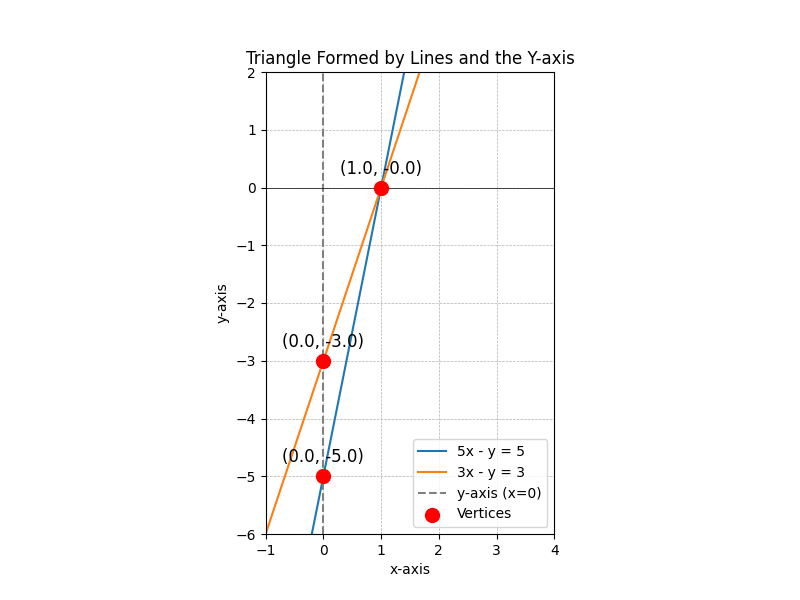
\includegraphics[width=0.75\columnwidth]{figs/1.png}
    \caption{Figure for 5.8.33}
\end{figure}

\end{document}
